%\chapter{Background}  \label{background}
\chapter{Background: Abstract Syntax Trees and Anti-unification}  \label{background1}

A programming language is described by the combination of its syntax and semantics. The syntax concerns the legal structures of programs written in the programming language, while the semantics is about the meaning of every construct in that language. Furthermore, the abstract syntactic structure of source code written in a programming language can be represented as an \emph{abstract syntax tree} (AST), in which nodes are occurrences of syntactic structures and edges represent nesting relationships. Since ASTs will be the form in which we represent and analyze source code, we need a means to generalize sets of ASTs in order to understand their commonalities while abstracting away their differences.  The theoretical framework of anti-unification is presented as that means.

In this chapter, ASTs are described briefly in Section~\ref{AST}, along with their more concrete counterparts, concrete syntax trees. Anti-unification is summarized in Section~\ref{AU}, starting with its most basic form, first-order anti-unification, and progressing to the form that we will make use of, higher-order anti-unification modulo equational theories.

\section{Concrete syntax trees and abstract syntax trees}\label{AST}

A concrete syntax tree is a tree (i.e., a kind of graph) $T=(V,E)$ whose vertices $V$ (equivalently, nodes) represent the syntactic structures (equivalently, syntactic elements) of a specific program written in a specific programming language and whose directed edges $E$ represent the nesting relationships amongst those syntactic structures.  Non-leaf nodes in a concrete syntax tree (also called a parse tree) represent the grammar productions that were satisfied in parsing the program it represents; leaf nodes represent the concrete lexemes, such as literals and keywords.

We focus on the Java programming language and we make use of the grammar in the language specification \cite[][Chapter 18]{2012:book:gosling} to determine the form of the concrete syntax trees.  Non-leaf node names are represented by names in ``camel-case'' written in italics.  Consider the trivial program in Figure~\ref{fig:java-example}; its concrete syntax tree is represented in Figure~\ref{fig:java-example-cst}.

\begin{figure}
\begin{lstlisting}
public class HelloWorld {
    public static void main(String[] args) {
        System.out.println("Hello world!");
    }
}
\end{lstlisting}
\caption{A simple example Java program.\label{fig:java-example}}
\end{figure}

\begin{sidewaysfigure}
\centering\resizebox{!}{0.65\textheight}{%
\begin{tikzpicture}
\node(cu) at (-14,20) {\textit{CompilationUnit}};
%
\node(td) at (-14,19) {\textit{TypeDeclaration}};
\draw[->](cu) -- (td) {};
%
\node(cid) at (-14,18) {\textit{ClassOrInterfaceDeclaration}};
\draw[->](td) -- (cid) {};
%
\node(mod2) at (-16,17) {\textit{Modifier}};
\draw[->](cid) -- (mod2) {};
%
\node(public2) at (-16,16) {\textsf{\small public}};
\draw[->](mod2) -- (public2) {};
%
\node(cd) at (-12,17) {\textit{ClassDeclaration}};
\draw[->](cid) -- (cd) {};
%
\node(ncd) at (-12,16) {\textit{NormalClassDeclaration}};
\draw[->](cd) -- (ncd) {};
%
\node(class) at (-16,15) {\textsf{\small class}};
\node(id7) at (-14,15) {\textit{Identifier}};
\node(cbody) at (-8,15) {\textit{ClassBody}};
\draw[->](ncd) -- (class) {};
\draw[->](ncd) -- (id7) {};
\draw[->](ncd) -- (cbody) {};
%
\node(HelloWorld) at (-14,14) {\textsf{\small HelloWorld}};
\draw[->](id7) -- (HelloWorld) {};
%
\node(obr2) at (-12,14) {\textsf{\small \{}};
\node(cbd) at (-8,14) {\textit{ClassBodyDeclaration}};
\node(cbr2) at (-4,14) {\textsf{\small \}}};
\draw[->](cbody) -- (obr2) {};
\draw[->](cbody) -- (cbd) {};
\draw[->](cbody) -- (cbr2) {};
%
\node(mod1) at (-12,13) {\textit{Modifier}};
\node(mod2) at (-10,13) {\textit{Modifier}};
\node(md) at (-4,13) {\textit{MemberDecl}};
\draw[->](cbd) -- (mod1) {};
\draw[->](cbd) -- (mod2) {};
\draw[->](cbd) -- (md) {};
%
\node(public1) at (-12,12) {\textsf{\small public}};
\draw[->](mod1) -- (public1) {};
%
\node(static) at (-10,12) {\textsf{\small static}};
\draw[->](mod2) -- (static) {};
%
\node(void) at (-8,12) {\textsf{\small void}};
\node(id6) at (-6,12) {\textit{Identifier}};
\node(vmdr) at (2,12) {\textit{VoidMethodDeclaratorRest}};
\draw[->](md) -- (void) {};
\draw[->](md) -- (id6) {};
\draw[->](md) -- (vmdr) {};
%
\node(main) at (-6,11) {\textsf{\small main}};
\draw[->](id6) -- (main) {};
%
\node(formals) at (-2,11) {\textit{FormalParameters}};
\draw[->](vmdr) -- (formals) {};
%
\node(op2) at (-5,10) {\textsf{\small (}};
\node(fpd) at (-2,10) {\textit{FormalParameterDecls}};
\node(cp2) at (1,10) {\textsf{\small )}};
\draw[->](formals) -- (op2) {};
\draw[->](formals) -- (fpd) {};
\draw[->](formals) -- (cp2) {};
%
\node(type) at (-4,9) {\textit{Type}};
\node(fpdr) at (0,9) {\textit{FormalParameterDeclsRest}};
\draw[->](fpd) -- (type) {};
\draw[->](fpd) -- (fpdr) {};
%
\node(rt) at (-6,8) {\textit{ReferenceType}};
\node(obt) at (-4,8) {\textsf{\small [}};
\node(cbt) at (-3,8) {\textsf{\small ]}};
\draw[->](type) -- (rt) {};
\draw[->](type) -- (obt) {};
\draw[->](type) -- (cbt) {};
%
\node(id5) at (-6,7) {\textit{Identifier}};
\draw[->](rt) -- (id5) {};
%
\node(String) at (-6,6) {\textsf{\small String}};
\draw[->](rt) -- (String) {};
%
\node(vdi) at (0,8) {\textit{VariableDeclaratorId}};
\draw[->](fpdr) -- (vdi) {};
%
\node(id4) at (0,7) {\textit{Identifier}};
\draw[->](vdi) -- (id4) {};
%
\node(args) at (0,6) {\textsf{\small args}};
\draw[->](id4) -- (args) {};
%
\node(block) at (6,11) {\textit{Block}};
\draw[->](vmdr) -- (block) {};
%
\node(obrace1) at (4,10) {\textsf{\small \{}};
\node(bs1) at (6,10) {\textit{BlockStatements}};
\node(cbrace1) at (8,10) {\textsf{\small \}}};
\draw[->](block) -- (obrace1) {};
\draw[->](block) -- (bs1) {};
\draw[->](block) -- (cbrace1) {};
%
\node(bs2) at (6,9) {\textit{BlockStatement}};
\draw[->](bs1) -- (bs2) {};
%
\node(stat) at (6,8) {\textit{Statement}};
\draw[->](bs2) -- (stat) {};
%
\node(se) at (5,7) {\textit{StatementExpression}};
\node(sc) at (7.5,7) {\textsf{\small ;}};
\draw[->](stat) -- (se) {};
\draw[->](stat) -- (sc) {};
%
\node(expr) at (5,6) {\textit{Expression}};
\draw[->](se) -- (expr) {};
%
\node(e1) at (5,5) {\textit{Expression1}};
\draw[->](expr) -- (e1) {};
%
\node(e2) at (5,4) {\textit{Expression2}};
\draw[->](e1) -- (e2) {};
%
\node(e3) at (5,3) {\textit{Expression3}};
\draw[->](e2) -- (e3) {};
%
\node(prim1) at (2,2) {\textit{Primary}};
\node(sel) at (8,2) {\textit{Selector}};
\draw[->](e3) -- (prim1) {};
\draw[->](e3) -- (sel) {};
%
\node(id1) at (0,1) {\textit{Identifier}};
\node(dot1) at (2,1) {\textsf{\small .}};
\node(id2) at (4,1) {\textit{Identifier}};
\draw[->](prim1) -- (id1) {};
\draw[->](prim1) -- (dot1) {};
\draw[->](prim1) -- (id2) {};
%
\node(dot2) at (6,1) {\textsf{\small .}};
\node(id3) at (8,1) {\textit{Identifier}};
\node(arguments) at (10,1) {\textit{Arguments}};
\draw[->](sel) -- (dot2) {};
\draw[->](sel) -- (id3) {};
\draw[->](sel) -- (arguments) {};
%
\node(System) at (0,0) {\textsf{\small System}};
\draw[->](id1) -- (System) {};
%
\node(out) at (4,0) {\textsf{\small out}};
\draw[->](id2) -- (out) {};
%
\node(println) at (8,0) {\textsf{\small println}};
\draw[->](id3) -- (println) {};
%
\node(op) at (8.5,0) {\textsf{\small (}};
\node(sl) at (10,0) {\textsf{\small "Hello world!"}};
\node(cp) at (11.5,0) {\textsf{\small )}};
\draw[->](arguments) -- (op) {};
\draw[->](arguments) -- (sl) {};
\draw[->](arguments) -- (cp) {};
\end{tikzpicture}%
}
\caption{The concrete syntax tree for the program of Figure~\ref{fig:java-example}.\label{fig:java-example-cst}}
\end{sidewaysfigure}

Beyond the fact that the concrete syntax tree is rather verbose and thus occupies a lot of space even for a trivial example, we can see two key problems with it: (1)~there are a multitude of redundant nodes such as \textit{Expression1}, \textit{Expression2}, and \textit{Expression3} that are present solely for purposes of creating an unambiguous grammar; and (2)~there are no nodes that express the concepts of ``method declaration'' and ``method invocation'' that should be obviously present in the example program.

To address these problems, concrete syntax trees are converted to abstract syntax trees (ASTs). An AST is similar in concept to a concrete syntax tree but it does not generally represent the parsing steps typed to differentiate different kinds of syntactic structure.  The node types are chosen to represent syntactical concepts; we use the grammar presented for exposition by \citet{2012:book:gosling}, which differs markedly from the grammar they propose in Chapter~18 for efficient parsing. Note that a given node type constrains the kinds and numbers of child nodes that it possesses.  The AST derived from the concrete syntax tree of Figure~\ref{fig:java-example-cst} is shown in Figure~\ref{fig:java-example-ast}.  Note that, although we know that (for any normal program), \code{System} refers to the class \code{java.lang.System} and \code{out} is a static field on that class; however, non-normal programs can occur and a pure syntactic analysis cannot rule out that \code{System} is a package and that \code{out} is a class therein declaring a static method \code{println(String)}.

\begin{sidewaysfigure}
\centering\resizebox{!}{0.4\textheight}{%
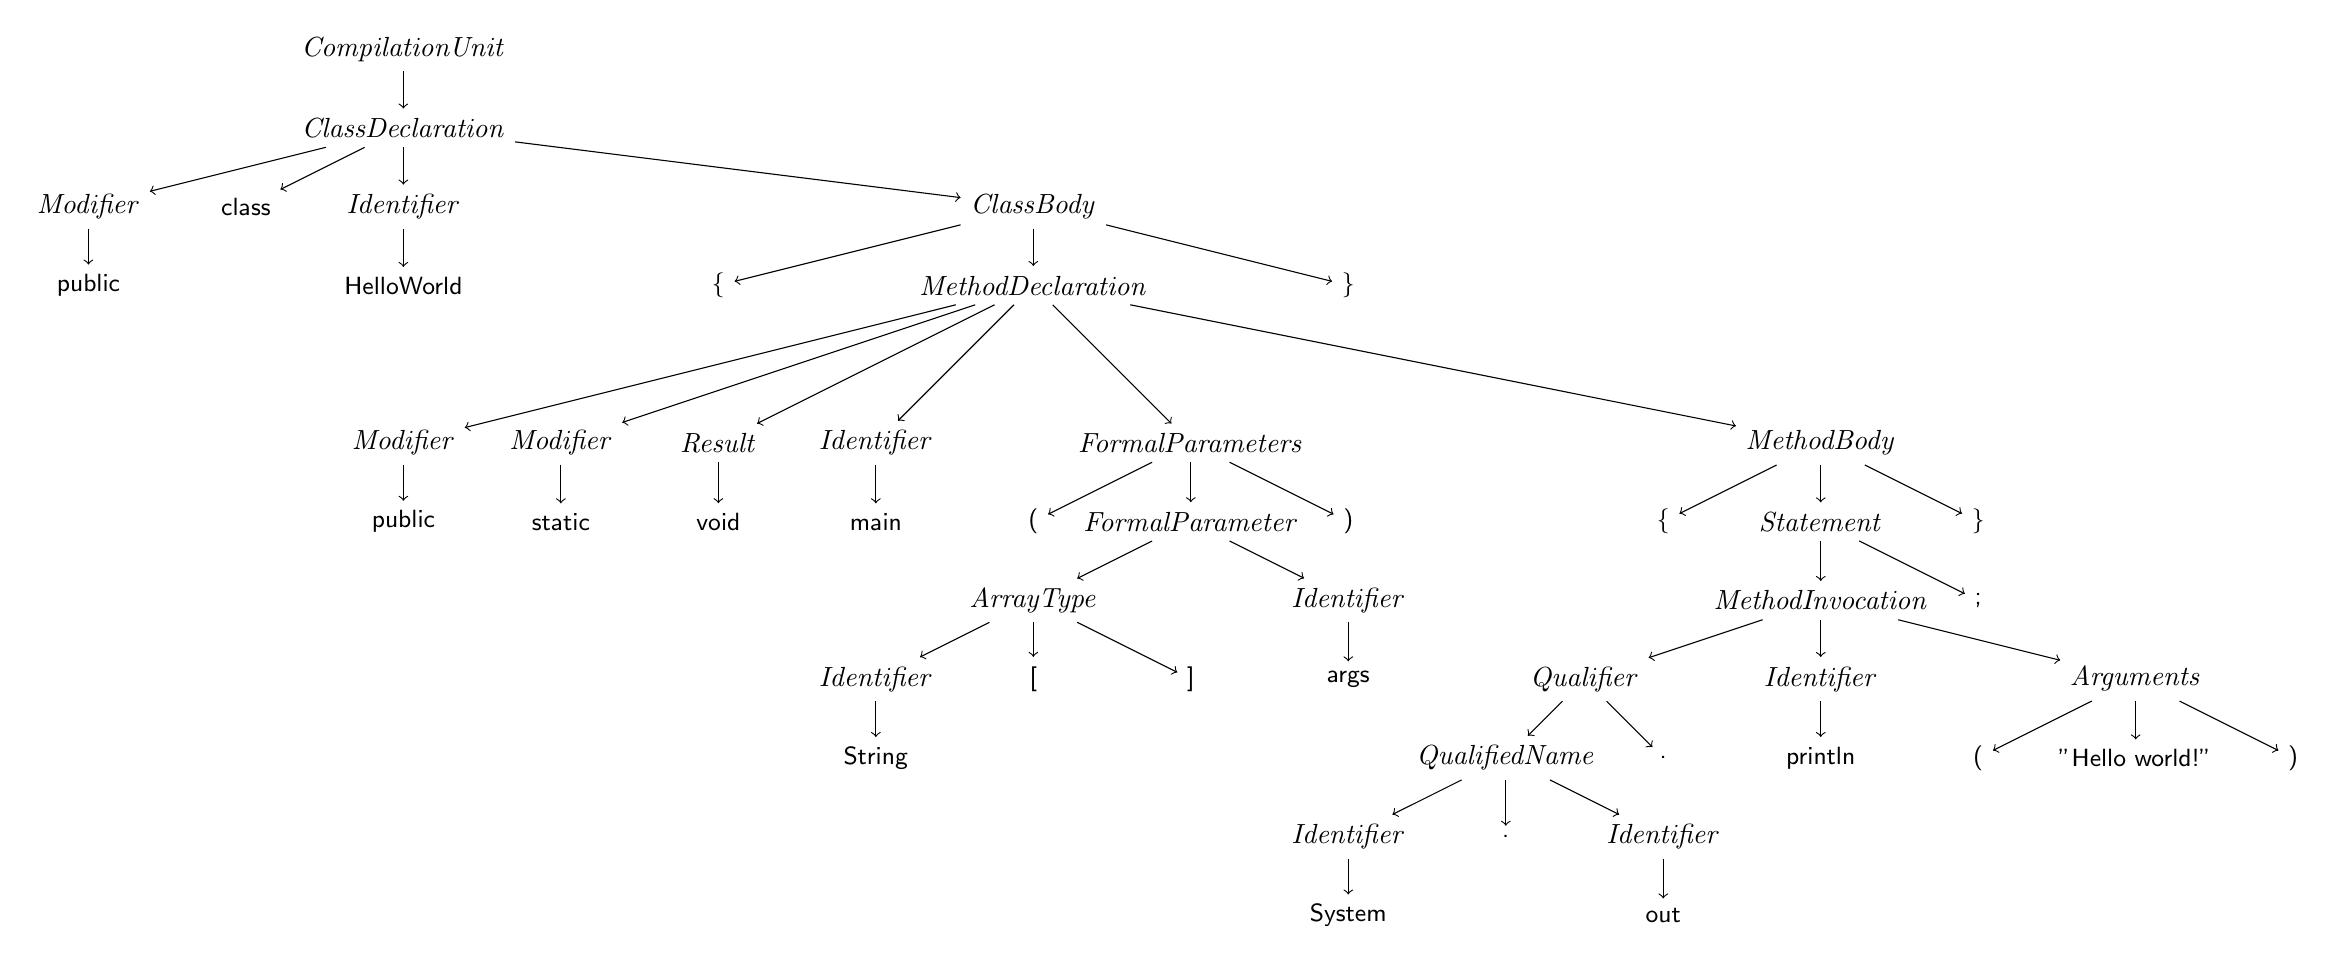
\begin{tikzpicture}
\node(cu) at (-12,11) {\textit{CompilationUnit}};
%
\node(cd) at (-12,10) {\textit{ClassDeclaration}};
\draw[->](cu) -- (cd) {};
%
\node(mod3) at (-16,9) {\textit{Modifier}};
\node(class) at (-14,9) {\textsf{\small class}};
\node(id7) at (-12,9) {\textit{Identifier}};
\node(cbody) at (-4,9) {\textit{ClassBody}};
\draw[->](cd) -- (mod3) {};
\draw[->](cd) -- (class) {};
\draw[->](cd) -- (id7) {};
\draw[->](cd) -- (cbody) {};
%
\node(public2) at (-16,8) {\textsf{\small public}};
\draw[->](mod3) -- (public2) {};
%
\node(HelloWorld) at (-12,8) {\textsf{\small HelloWorld}};
\draw[->](id7) -- (HelloWorld) {};
%
\node(obr2) at (-8,8) {\textsf{\small \{}};
\node(md) at (-4,8) {\textit{MethodDeclaration}};
\node(cbr2) at (0,8) {\textsf{\small \}}};
\draw[->](cbody) -- (obr2) {};
\draw[->](cbody) -- (md) {};
\draw[->](cbody) -- (cbr2) {};
%
\node(mod1) at (-12,6) {\textit{Modifier}};
\node(mod2) at (-10,6) {\textit{Modifier}};
\node(result) at (-8,6) {\textit{Result}};
\node(id6) at (-6,6) {\textit{Identifier}};
\node(fps) at (-2,6) {\textit{FormalParameters}};
\node(mbody) at (6,6) {\textit{MethodBody}};
\draw[->](md) -- (mod1) {};
\draw[->](md) -- (mod2) {};
\draw[->](md) -- (result) {};
\draw[->](md) -- (id6) {};
\draw[->](md) -- (fps) {};
\draw[->](md) -- (mbody) {};
%
\node(public1) at (-12,5) {\textsf{\small public}};
\draw[->](mod1) -- (public1) {};
%
\node(static) at (-10,5) {\textsf{\small static}};
\draw[->](mod2) -- (static) {};
%
\node(void) at (-8,5) {\textsf{\small void}};
\draw[->](result) -- (void) {};
%
\node(main) at (-6,5) {\textsf{\small main}};
\draw[->](id6) -- (main) {};
%
\node(op2) at (-4,5) {\textsf{\small (}};
\node(fp) at (-2,5) {\textit{FormalParameter}};
\node(cp2) at (0,5) {\textsf{\small )}};
\draw[->](fps) -- (op2) {};
\draw[->](fps) -- (fp) {};
\draw[->](fps) -- (cp2) {};
%
\node(type) at (-4,4) {\textit{ArrayType}};
\node(id5) at (0,4) {\textit{Identifier}};
\draw[->](fp) -- (type) {};
\draw[->](fp) -- (id5) {};
%
\node(id4) at (-6,3) {\textit{Identifier}};
\node(obt) at (-4,3) {\textsf{\small [}};
\node(cbt) at (-2,3) {\textsf{\small ]}};
\node(args) at (0,3) {\textsf{\small args}};
\draw[->](type) -- (id4) {};
\draw[->](type) -- (obt) {};
\draw[->](type) -- (cbt) {};
\draw[->](id5) -- (args) {};
%
\node(String) at (-6,2) {\textsf{\small String}};
\draw[->](id4) -- (String) {};
%
\node(obrace1) at (4,5) {\textsf{\small \{}};
\node(stat) at (6,5) {\textit{Statement}};
\node(cbrace1) at (8,5) {\textsf{\small \}}};
\draw[->](mbody) -- (obrace1) {};
\draw[->](mbody) -- (stat) {};
\draw[->](mbody) -- (cbrace1) {};
%
\node(mi) at (6,4) {\textit{MethodInvocation}};
\node(sc) at (8,4) {\textsf{\small ;}};
\draw[->](stat) -- (mi) {};
\draw[->](stat) -- (sc) {};
%
%
\node(qual) at (3,3) {\textit{Qualifier}};
\node(id3) at (6,3) {\textit{Identifier}};
\node(arguments) at (10,3) {\textit{Arguments}};
\draw[->](mi) -- (qual) {};
\draw[->](mi) -- (id3) {};
\draw[->](mi) -- (arguments) {};
%
\node(qn) at (2,2) {\textit{QualifiedName}};
\node(dot2) at (4,2) {\textsf{\small .}};
\node(println) at (6,2) {\textsf{\small println}};
\node(op) at (8,2) {\textsf{\small (}};
\node(sl) at (10,2) {\textsf{\small "Hello world!"}};
\node(cp) at (12,2) {\textsf{\small )}};
\draw[->](qual) -- (qn) {};
\draw[->](qual) -- (dot2) {};
\draw[->](id3) -- (println) {};
\draw[->](arguments) -- (op) {};
\draw[->](arguments) -- (sl) {};
\draw[->](arguments) -- (cp) {};
%
\node(id1) at (0,1) {\textit{Identifier}};
\node(dot1) at (2,1) {\textsf{\small .}};
\node(id2) at (4,1) {\textit{Identifier}};
\draw[->](qn) -- (id1) {};
\draw[->](qn) -- (dot1) {};
\draw[->](qn) -- (id2) {};
%
\node(System) at (0,0) {\textsf{\small System}};
\draw[->](id1) -- (System) {};
%
\node(out) at (4,0) {\textsf{\small out}};
\draw[->](id2) -- (out) {};
\end{tikzpicture}%
}
\caption{The abstract syntax tree derived from the concrete syntax tree of Figure~\ref{fig:java-example-cst}.\label{fig:java-example-ast}}
\end{sidewaysfigure}

This is still verbose, so in practice we elide details that are implied or otherwise trivial, to arrive at a more abstract AST as shown in Figure~\ref{fig:java-example-ast2}.

\begin{sidewaysfigure}
\centering\resizebox{!}{0.4\textheight}{%
\begin{tikzpicture}
\node(cu) at (-12,11) {\textit{CompilationUnit}};
%
\node(cd) at (-12,10) {\textit{ClassDeclaration}};
\draw[->](cu) -- (cd) {};
%
\node(HelloWorld) at (-12,8) {\textsf{\small HelloWorld}};
\draw[->](cd) -- (HelloWorld) {};
%
\node(md) at (-4,8) {\textit{MethodDeclaration}};
\draw[->](cd) -- (md) {};
%
\node(result) at (-8,6) {\textit{Result}};
\node(fps) at (-2,6) {\textit{FormalParameters}};
\node(mbody) at (6,6) {\textit{MethodBody}};
\draw[->](md) -- (result) {};
\draw[->](md) -- (fps) {};
\draw[->](md) -- (mbody) {};
%
\node(void) at (-8,5) {\textsf{\small void}};
\draw[->](result) -- (void) {};
%
\node(main) at (-6,5) {\textsf{\small main}};
\draw[->](md) -- (main) {};
%
\node(fp) at (-2,5) {\textit{FormalParameter}};
\draw[->](fps) -- (fp) {};
%
\node(type) at (-4,4) {\textit{ArrayType}};
\draw[->](fp) -- (type) {};
%
\node(args) at (0,3) {\textsf{\small args}};
\draw[->](fp) -- (args) {};
%
\node(String) at (-6,2) {\textsf{\small String}};
\draw[->](type) -- (String) {};
%
\node(mi) at (6,4) {\textit{MethodInvocation}};
\draw[->](mbody) -- (mi) {};
%
\node(arguments) at (10,3) {\textit{Arguments}};
\draw[->](mi) -- (arguments) {};
%
\node(qn) at (2,2) {\textit{QualifiedName}};
\node(dot2) at (4,2) {\textsf{\small .}};
\node(println) at (6,2) {\textsf{\small println}};
\node(sl) at (10,2) {\textsf{\small "Hello world!"}};
\draw[->](mi) -- (qn) {};
\draw[->](mi) -- (println) {};
\draw[->](arguments) -- (sl) {};
%
\node(System) at (0,0) {\textsf{\small System}};
\draw[->](qn) -- (System) {};
%
\node(out) at (4,0) {\textsf{\small out}};
\draw[->](qn) -- (out) {};
\end{tikzpicture}%
}
\caption{A more abstract, abstract syntax tree derived from the concrete syntax tree of Figure~\ref{fig:java-example-cst}.\label{fig:java-example-ast2}}
\end{sidewaysfigure}

\section{First-order anti-unification}   \label{AU}

This section defines terms, substitutions, applying a substitution to a term, and instances and anti-instances of a term, as the requirements needed  to describe anti-unification theory (and its dual, unification theory).

\begin{defn}[Term]\label{def:term}
A term is defined to be a variable, a constant, or a function symbol followed by a list of terms as the arguments of the function.  [Note that function symbols without the subsequent list of terms do not constitute terms.]
\end{defn}

Function symbols taking $n$ arguments are called $n$-ary function symbols; 0-ary function symbols are called constants. The identifiers starting with a lowercase letter are used to represent function symbols (e.g., $f(a,b)$, $g(a,b)$) and constants (e.g., $a$, $b$), while variables are represented by identifiers starting with an uppercase letter (e.g., $X$, $Y$). The following are examples of a term:
\begin{itemize} [leftmargin=0.7in]
\item $Y$
\item $a$
\item $f(X, c)$
\item $f(g(X, b),Y, g(a, Z))$
\end{itemize}
%A term is called grounded if it does not contain any variables (e.g., $f(a,b)}), and
Note that for any term there is a unique, equivalent tree and vice versa: constants and (first-order) variables are leaf nodes, while function symbols are non-leaf nodes; a function with given arguments is represented by a non-leaf node (representing the function symbol) with directed edges pointing to leaf nodes representing each argument.  For example:
\begin{itemize} [leftmargin=0.7in]
\item $Y$
\item $a$
\item $X \leftarrow f \rightarrow c$
\item \begin{tikzpicture}
\node(f) at (3,2) {$f$};
\node(g1) at (1,1) {$g$};
\node(Y) at (3,1) {$Y$};
\node(g2) at (5,1) {$g$};
\node(X) at (0,0) {$X$};
\node(b) at (2,0) {$b$};
\node(a) at (4,0) {$a$};
\node(Z) at (6,0) {$Z$};
%
\draw[->](f) -- (g1) {};
\draw[->](f) -- (Y) {};
\draw[->](f) -- (g2) {};
\draw[->](g1) -- (X) {};
\draw[->](g1) -- (b) {};
\draw[->](g2) -- (a) {};
\draw[->](g2) -- (Z) {};
\end{tikzpicture}
\end{itemize}

\begin{defn}[Substitution]\label{def:substitution}
A substitution is a set of mappings, each from a variable to a term.
\end{defn}

\begin{defn}[Applying a substitution]\label{def:substitution}
Applying a substitution to a term results in the replacement of all occurrences of each variable in the term, by its corresponding term as defined in the substitution.
\end{defn}

As an example, applying the substitution $\Theta$ = ({$X \rightarrow a, Y \rightarrow b $})
to the term $f(X,Y)$ results in the replacement of all occurrences of the variable $X$ by the term $a$ and all occurrences of the variable $Y$ by the term $b$, and thus $f(X,Y)\xrightarrow{\Theta} f(a,b)$.

\begin{defn}[Instance \& anti-instance]\label{def:instance}
$a$ is an instance of a term $X$ and $X$ is an anti-instance of $a$, if there is a substitution $\Theta$ such that the application of $\Theta$ on $X$ results in $a$ ($X\xrightarrow{\Theta}a$).
\end{defn}

\begin{defn}[Unifier]\label{def:unifier}
A unifier is a common instance of two given terms.
\end{defn}

Unification usually aims to create the \emph{most general unifier} (MGU); that is, $U$ is the MGU of two terms such that for all unifiers $U'$ there exists a substitution $\Theta$ such that $U\xrightarrow{\Theta}U'$. Unification aims to make a more concrete structure in essence, whereas what we need is a more generalized structure, which leads to the use of the dual of unification, called \emph{anti-unification}.

\begin{defn}[Anti-unifier]\label{def:generalization}
$X$ is an anti-unifier (or generalization) for $a$ and $b$, if $X$ is an anti-instance for $a$ and an anti-instance for $b$ under substitutions $\Theta_1$ and $\Theta_2$, respectively ($X\xrightarrow{\Theta_1}a$ and $X\xrightarrow{\Theta_2}b$).
\end{defn}

An anti-unifier contains common pieces of the original terms, while the differences are abstracted away using variables. An anti-unifier for a pair of terms always exists since we can anti-unify any two terms by the anti-instance $X$, i.e., a single variable. However, anti-unification usually aims to find the \emph{most specific anti-unifier} (MSA), that is, $A$ is the MSA of two structures where there exists no anti-unifier $A'$ such that $A\xrightarrow{\Theta}A'$.

As an example, the anti-unifier of two given terms $f(X,b)$ and $f(a,Y)$ is the new term $f(X,Y)$, containing common pieces of the two original terms. The variable $Y$ in the anti-unifier $f(X,Y)$ can be substituted by the term $b$ to re-create $f(X,b)$ (with $\Theta_1 = Y\xrightarrow{}b$) and the variable $X$ in the anti-unifier can be substituted by the term $a$ to re-create $f(a,Y)$
(with $\Theta_2 = X\xrightarrow{\Theta}a$), as depicted in Figure~\ref{fig:uni-anti-uni}.
In addition, the unifier $f(a,b)$ of the two terms can be instantiated by applying the substitutions $\Theta_1'=X\xrightarrow{\Theta}a$ and $\Theta_2'=Y\xrightarrow{\Theta}b$ on the terms $f(X,b)$ and $f(a,Y)$, respectively.

\begin{figure} [t]
\centering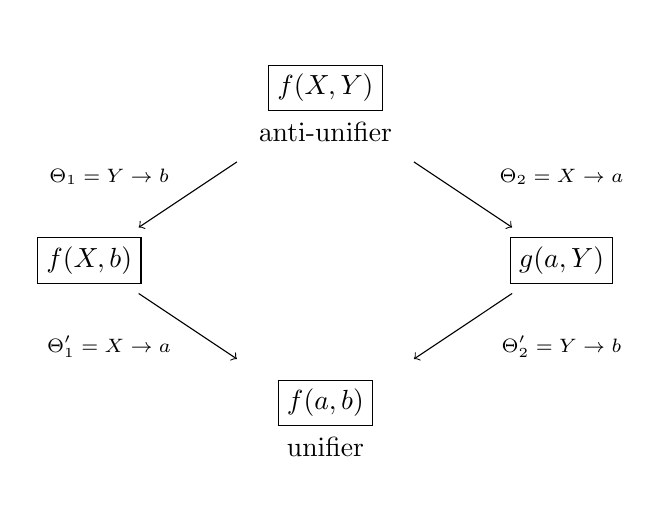
\begin{tikzpicture}
\node(au) at (5,2) {\parbox{2cm}{\begin{center}\fbox{$f(X,Y)$}\\*[3pt]\text{anti-unifier}\end{center}}};
\node(left) at (2,0) {\fbox{\mbox{$f(X,b)$}}};
\node(right) at (8,0) {\fbox{\mbox{$g(a,Y)$}}};
\node(u) at (5,-2) {\parbox{2cm}{\begin{center}\fbox{$f(a,b)$}\\*[3pt]\text{unifier}\end{center}}};
%
\draw[->](au) -- (left) node[pos=0.5, above]{\mbox{\scriptsize $\Theta_1 = Y \rightarrow b$\hspace*{2cm}}};
\draw[->](au) -- (right) node[pos=0.5, above]{\mbox{\hspace*{2.5cm}\scriptsize $\Theta_2 = X \rightarrow a$}};
\draw[->](left) -- (u) node[pos=0.5, below]{\mbox{\scriptsize $\Theta_1' = X \rightarrow a$\hspace*{2cm}}};
\draw[->](right) -- (u) node[pos=0.5, below]{\mbox{\hspace*{2.5cm}\scriptsize $\Theta_2' = Y \rightarrow b$}};
\end{tikzpicture}
%  {\makecell[l]{\hspace{0.4cm}f(X,Y)\\\text{anti-unifier}}}
%  \arrow{dr}{\Theta_2 = X \rightarrow a}
%  \arrow[->,swap]{dl}{\Theta_1 = Y \rightarrow b} % <-- reflect the direction of the hook
%\\
%f(X,b)
% \arrow[->,swap]{dr}{\Theta_1' = X \rightarrow a}
% %\arrow{dr}
%&&
%f(a, Y)
%  \arrow{dl}{\Theta_2' = Y \rightarrow b}
%  \\
%&
%{\makecell[l]{f(a,b)\\\text{unifier}}}
%\end{tikzcd}
%\]
  \caption{Unification and anti-unification of the terms $f(X,b)$ and $f(a,Y)$.}
  \label{fig:uni-anti-uni}
\end{figure}

The MSA should preserve as much of common pieces of both original terms as possible; however, first-order anti-unification fails to capture complex commonalities as it restricts substitutions to only replace first-order variables by terms. That is, when two terms differ in function symbols, first-order anti-unification fails to capture common details of them. For example, the first-order anti-unifier of the terms $f(a,b)$ and $g(a,b)$ is $X$ as depicted in Figure~\ref{fig:first-anti-uni}.

\begin{figure}[t]
\centering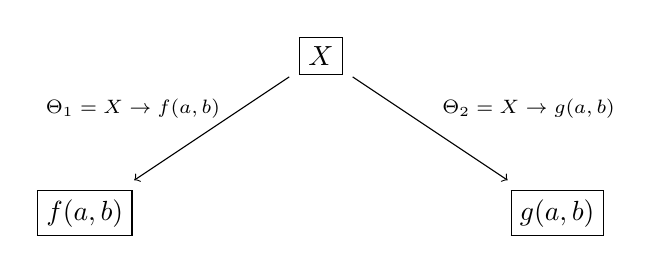
\begin{tikzpicture}
\node(au) at (5,2) {\fbox{\mbox{$X$}}};
\node(left) at (2,0) {\fbox{\mbox{$f(a,b)$}}};
\node(right) at (8,0) {\fbox{\mbox{$g(a,b)$}}};
%
\draw[->](au) -- (left) node[pos=0.5, above]{\mbox{\scriptsize $\Theta_1 = X \rightarrow f(a,b)$\hspace*{2cm}}};
\draw[->](au) -- (right) node[pos=0.5, above]{\mbox{\hspace*{2.5cm}\scriptsize $\Theta_2 = X \rightarrow g(a,b)$}};
\end{tikzpicture}
\caption{First-order anti-unification of the terms $f(a,b)$ and $g(a,b)$.\label{fig:first-anti-uni}}
\end{figure}

Higher-order anti-unification would allow us to create the MSA by extending the set of possible substitutions such that variables can be replaced not only by terms but also by function symbols in order to retain the detailed commonalities. For example, the higher-order anti-unifier of the terms $f(a,b)$ and $g(a,b)$ is $X(a,b)$ as depicted in Figure~\ref{fig:higher-anti-uni}.
\begin{figure}[t]
\centering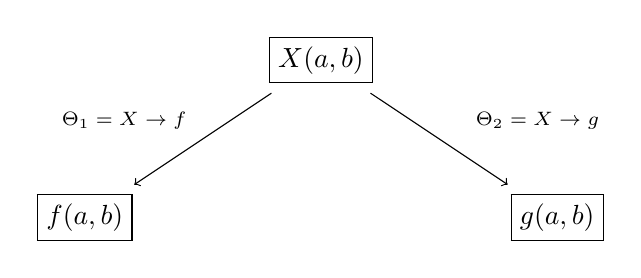
\begin{tikzpicture}
\node(au) at (5,2) {\fbox{\mbox{$X(a,b)$}}};
\node(left) at (2,0) {\fbox{\mbox{$f(a,b)$}}};
\node(right) at (8,0) {\fbox{\mbox{$g(a,b)$}}};
%
\draw[->](au) -- (left) node[pos=0.5, above]{\mbox{\scriptsize $\Theta_1 = X \rightarrow f$\hspace*{2cm}}};
\draw[->](au) -- (right) node[pos=0.5, above]{\mbox{\hspace*{2.5cm}\scriptsize $\Theta_2 = X \rightarrow g$}};
\end{tikzpicture}
\caption{Higher-order anti-unification of the terms $f(a,b)$ and $g(a,b)$.\label{fig:higher-anti-uni}}
\end{figure}

\section{Higher-Order Anti-unification Modulo Equational Theories}\label{HOAUMT}

%\begin{align}
%\Theta_1 = (W &\rightarrow \text{ \textsf{\small WARNING}},\nonumber\\
%X &\rightarrow \text{ \textit{methodCall}(\textit{simpleName}(\textsf{\small getClassName}), \textit{arguments}())},\nonumber\\
%Y &\rightarrow \text{ \textsf{\small "should extend EditPlugin not EBPlugin since it has an empty "}},\nonumber\\
%Z &\rightarrow \text{ \textit{methodCall}(\textit{simpleName}(\textsf{\small handleMessage}), \textit{arguments}())})\label{eq:theta1}\\
%\Theta_2 = (W &\rightarrow \text{ \textsf{\small ERROR}},\nonumber\\
%X &\rightarrow \text{ \NIL{}},\nonumber\\
%Y &\rightarrow \text{ \textsf{\small "Unknown action: "}},\nonumber\\
%Z &\rightarrow \text{ \textit{simpleName}(\textsf{\small actionName})})\label{eq:theta2}
%\end{align}
%
%%\item it can be mapped to our recursive definition of a term, where AST nodes and simple values may be viewed as function-symbols and constants, respectively
%
%\begin{figure}[p]
%\begin{small}
%\begin{tikzpicture}
%\node(a) at (4.25,10) {%
%\fbox{\parbox[b][][b]{3in}{%
%\text{\textit{methodCall}(}\\
%\text{\hspace*{1em}\textit{qualifiedName}(\textsf{\footnotesize Log}, \textit{simpleName}(\textsf{\footnotesize log})),}\\
%\text{\hspace*{1em}\textit{arguments}(}\\
%\text{\hspace*{2em}\textit{qualifiedName}(\textsf{\footnotesize Log}, \textit{simpleName}(\textit{W})),}\\
%\text{\hspace*{2em}\textit{thisExpression}(),}\\
%\text{\hspace*{2em}\textit{additionExpression}(\textit{X}, \textit{stringLiteral}(\textit{Y}), \textit{Z})))}}}%
%};
%\node(b) at (0,0) {%
%\fbox{\parbox[t][][b]{3.1in}{%
%\text{\textit{methodCall}(}\\
%\text{\hspace*{1em}\textit{qualifiedName}(\textsf{\footnotesize Log}, \textit{simpleName}(\textsf{\footnotesize log})),}\\
%\text{\hspace*{1em}\textit{arguments}(}\\
%\text{\hspace*{2em}\textit{qualifiedName}(\textsf{\footnotesize Log},}\\ \text{\hspace*{3em}\mbox{\textit{simpleName}(\textsf{\footnotesize WARNING})}),}\\
%\text{\hspace*{2em}\textit{thisExpression}(),}\\
%\text{\hspace*{2em}\textit{additionExpression}(}\\
%\text{\hspace*{3em}\textit{methodCall}(\textit{simpleName}(\textsf{\footnotesize getClassName}),}\\ \text{\hspace*{4em}\textit{arguments}()),}\\
%\text{\hspace*{3em}\textit{stringLiteral}(\textsf{\footnotesize " should extend ... "}),}\\
%\text{\hspace*{3em}\textit{methodCall}(\textit{simpleName}(\textsf{\footnotesize handleMessage}),}\\ \text{\hspace*{4em}\textit{arguments}()))))}}}%
%};
%\node(c) at (8.5,0.7) {%
%\fbox{\parbox[t][][b]{2.55in}{%
%\text{\textit{methodCall}(}\\
%\text{\hspace*{1em}\textit{qualifiedName}(\textsf{\footnotesize Log}, \textit{simpleName}(\textsf{\footnotesize log})),}\\
%\text{\hspace*{1em}\textit{arguments}(}\\
%\text{\hspace*{2em}\textit{qualifiedName}(\textsf{\footnotesize Log},}\\ \text{\hspace*{3em}\mbox{\textit{simpleName}(\textsf{\footnotesize ERROR})}),}\\
%\text{\hspace*{2em}\textit{thisExpression}(),}\\
%\text{\hspace*{2em}\textit{additionExpression}(}\\
%\text{\hspace*{3em}\textit{stringLiteral}(\textsf{\footnotesize "Unknown action: "}),}\\
%\text{\hspace*{3em}\textit{simpleName}(\textsf{\footnotesize actionName}))))}}}%
%};
%
%\draw[->](a) -- (b) node[pos=0.5,above]{$\Theta_1\qquad$};
%\draw[->](a) -- (c) node[pos=0.5,above]{$\qquad\Theta_2$};
%\end{tikzpicture}
%\end{small}
%\caption{The anti-unification of the AUASTs of the logging calls in Examples 1 and 2.\label{fig:logging-anti}}
%\end{figure}
%%The AUASTs of log Method Invocation nodes from the Java classes in Figure~\ref{ch3-ex1} and Figure~\ref{ch3-ex2}.
%
%Applying higher-order anti-unification on AUAST structures could help to construct a structural generalization by maintaining the common pieces and abstracting the differences away using variables. However, it is not comprehensive enough to solve our problem as it does not consider background knowledge about AST structures, such as syntactically different but semantically relevant structures, missing structures, and different ordering of arguments. In the following section, we will look at an extension of anti-unification, higher-order anti-unification modulo theories, and how it can sufficiently address the limitations of anti-unification in our context.

%anti-unification cannot incorporate any background knowledge such as sematic knowledge required to solve our problem, and we should apply an extended form of anti-unification, called higher-order anti-unification modulo theories, where a set of equivalence equations is defined to incorporate semantic knowledge of structural equivalences supported by the Java language specification. An equivalence equation $=_E$ determines which terms are considered equal, and the set of equivalence equations must be applied on higher-order extended structures to allow the anti-unification of AST structures that are not identical but are semantically equivalent.
In higher-order anti-unification modulo (equational) theories, a set of equational theories, which treat different structures as equivalent, is defined to incorporate background knowledge. Each equational theory $=_E$ determines which terms are considered equal and a set of these equations can be applied on higher-order extended structures to determine structural equivalences. For example, we have introduced an equivalence equation $=_E$, such that $f(X,Y) =_E f(Y,X)$ to indicate that the ordering of arguments does not matter in our context.

% nil restriction!!!!
We have also introduced a theory, called \NIL{}-theory, that adds the concept of a \NIL{} structure, which permits a structure to be equated with nothing, and defines an equivalence equation $=_E$ for it. The \NIL{} structure can be used to anti-unify two structures when a substructure exists in one but is missing from the other. However, some requirements should be taken to avoid the overuse of \NIL{} structures such that the original structures must have common substructures but vary in the size for dissimilar substructures. For example, we can anti-unify the two structures $b$ and $f(a,b)$ through the application of \NIL{}-theory by creating the term $\NIL{}(\NIL{},b)$ which is $=_E$ to $f(b)$ and anti-unifying $\NIL{}(\NIL{},b)$ with $f(a,b)$ as depicted in Figure~\ref{fig:anti-nil}.
% to introduce an equivalence equation =E for the NIL structure
% it should be modified
% should it be different?
\begin{figure}[t]
\centering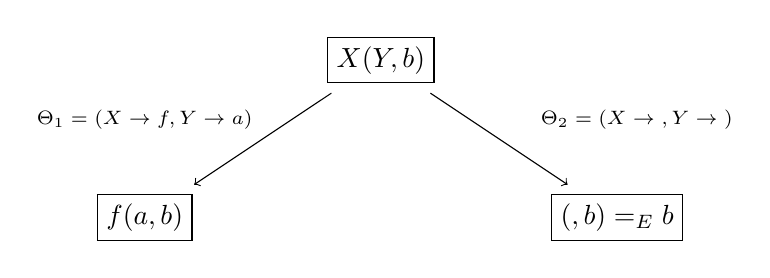
\begin{tikzpicture}
\node(au) at (5,2) {\fbox{\mbox{$X(Y,b)$}}};
\node(left) at (2,0) {\fbox{\mbox{$f(a,b)$}}};
\node(right) at (8,0) {\fbox{\mbox{$\NIL{}(\NIL{},b) =_E  b$}}};
%
\draw[->](au) -- (left) node[pos=0.5, above]{\mbox{\scriptsize $\Theta_1 = ( X \rightarrow f, Y \rightarrow a)$\hspace*{3cm}}};
\draw[->](au) -- (right) node[pos=0.5, above]{\mbox{\hspace*{3.5cm}\scriptsize $\Theta_2 = ( X \rightarrow \NIL{}, Y \rightarrow \NIL{})$}};
\end{tikzpicture}
\caption{Anti-unification of the terms $f(a, b)$ and $\NIL{}(\NIL{},b)$.\label{fig:anti-nil}}
\end{figure}


We have also defined a set of equivalence equations to incorporate semantic knowledge of structural equivalences supported by the Java language specification as it provides various ways to define the same language specifications. These theories should be applied on higher-order extended structures to anti-unify AST structures that are not identical but are semantically equivalent. For example, consider \code{for}- and \code{while}-statements that are two types of looping structure in Java programming language: they have different syntax but semantically cover the same concept. Let us look at the code snippets \code{for(i=0;i<10;i++)} and \code{while(i<10)}, whose ASTs can be represented as \code{for(}\textit{Initializer}(\code{i}, \code{0})\code{;} \textit{LessThanExpression}(\code{i}, \code{10})\code{;} \textit{Updaters}(\textit{PostIncrementExpression}(\code{i}))) and \code{while}(\textit{LessThanExpression}(\code{i}, \code{10})), respectively. We could define an equivalence equation $=_E$ that allows the anti-unification of \code{for}- and \code{while}-statements. We also need to utilize the \NIL{}-theory to handle the varying number of arguments as the \code{for}-loop has three arguments whereas the \code{while}-loop only has one. Using the \NIL{}-theory we can create the structure \code{while}(\NIL{}(\NIL{}, \NIL{}), \textit{LessThanExpression}(\code{i}, \code{10}), \NIL{}(\NIL{}, \NIL{})) that is $=_E$ to \code{while}(\textit{LessThanExpression}(\code{i}, \code{10})) and construct the anti-unifier, $V_0$($V_1$($V_2$, $V_3$), \textit{LessThanExpression}(\code{i}, \code{10}), $V_4$($V_5$($V_2$))), as depicted in Figure~\ref{fig:for-while}.

\begin{figure}[t]
\centering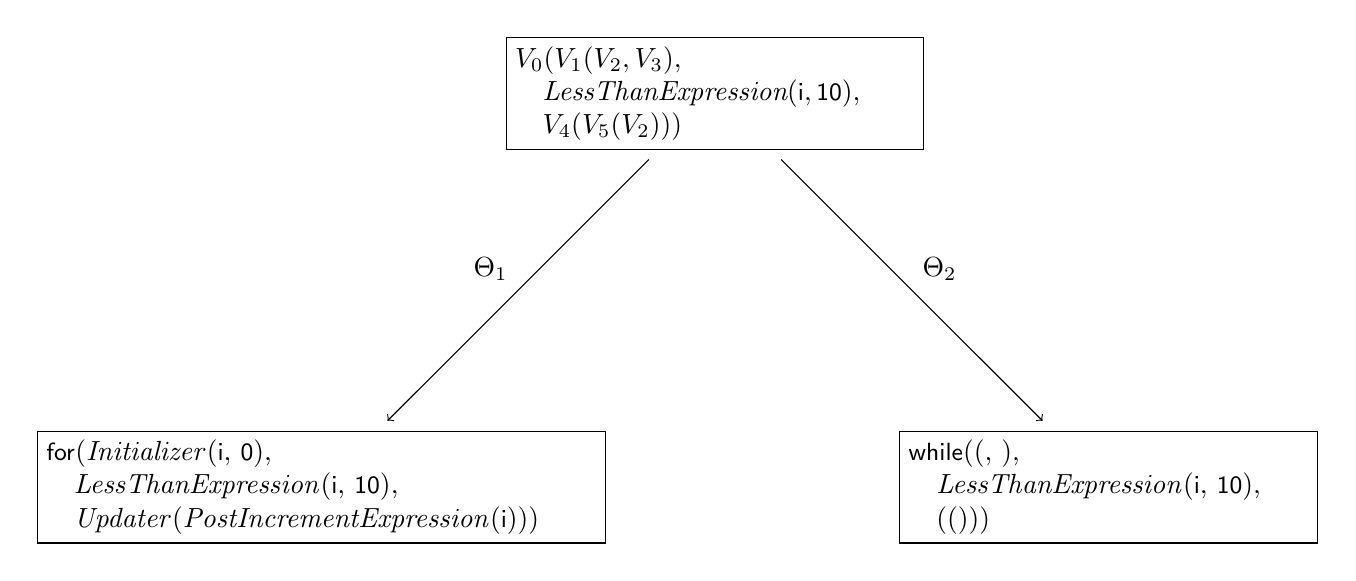
\begin{tikzpicture}
\node(au) at (5,5) {\fbox{\parbox{2in}{$V_0(V_1(V_2,V_3),$\\$\text{\quad\textit{LessThanExpression}(\textsf{\small i}, \textsf{\small 10})}$,\\ \mbox{$\quad V_4(V_5(V_2)))$}}}};
%
\node(left) at (0,0) {\fbox{\parbox{2.75in}{%
\textsf{\small for}(\textit{Initializer}(\textsf{\small i}, \textsf{\small 0}),\\\mbox{\quad\textit{LessThanExpression}}(\textsf{\small i}, \textsf{\small 10}),\\ \mbox{\quad\textit{Updater}}(\textit{PostIncrementExpression}(\textsf{\small i})))}}};
%
\node(right) at (10,0) {\fbox{\parbox{2in}{%
\textsf{\small while}(\NIL{}(\NIL{}, \NIL{}),\\ \mbox{\quad\textit{LessThanExpression}}(\textsf{\small i}, \textsf{\small 10}),\\ \mbox{\quad\NIL{}}(\NIL{}(\NIL{})))}}};
%
\draw[->](au) -- (right) node[pos=0.5, above]{$\qquad\Theta_2$};
%
\draw[->](au) -- (left) node[pos=0.5, above]{$\Theta_1\qquad$};
\end{tikzpicture}
\caption{The anti-unification of the structures \code{for}(\textit{Initializer}(\code{i}, \code{0}), \mbox{\textit{LessThanExpression}(\code{i}, \code{10}),} \textit{Updater}(\textit{PostIncrementExpression}(\code{i}))) and \code{while}(\NIL{}(\NIL{}, \NIL{}), \mbox{\textit{LessThanExpression}(\code{i}, \code{10}),} \NIL{}(\NIL{}, \NIL{})). The substitutions are defined as follows: $\Theta_1 = (V_0 \rightarrow \text{ \textsf{\small for}}, V_1 \rightarrow \text{ \textit{Initializer}}, V_2 \rightarrow \text{ \textsf{\small i}}, V_3 \rightarrow 0, V_4 \rightarrow \text{ \textit{Updater}}, V_5 \rightarrow \text{ \textit{PostIncrementExpression}})$; and $\Theta_2 = (V_0 \rightarrow \text{ \textsf{\small while}}, V_1 \rightarrow \text{ \NIL{}}, V_2 \rightarrow \text{ \NIL{}}, V_3 \rightarrow \text{ \NIL{}}, V_4 \rightarrow \text{ \NIL{}}, V_5 \rightarrow \text{ \NIL{}})$\label{fig:for-while}}
\end{figure}
% higher-order extension and the equational theories
% provide a better example

However, defining complex substitutions in higher-order anti-unification modulo theories results in losing the uniqueness of MSA. For example, consider the terms $f(g(a,e))$ and $f(g(a,b),$\linebreak$g(d,e))$. As described in Figure~\ref{fig:multipleMSA}, two MSAs exist for these terms: we can anti-unify $g(a,e)$ and $g(a,b)$ to create the anti-unifier $g(a,X_0)$ and anti-unify $g(d,e)$ with the NIL structure to create the anti-unifier $Y(Z,X_1)$; or we can anti-unify $g(a,e)$ and $g(d,e)$ to create the anti-unifier $g(X_0,e)$ and anti-unify $g(a,b)$ with the \NIL{} structure to create the anti-unifier $Y(Z,X_1)$.

\begin{figure}[t]
\centering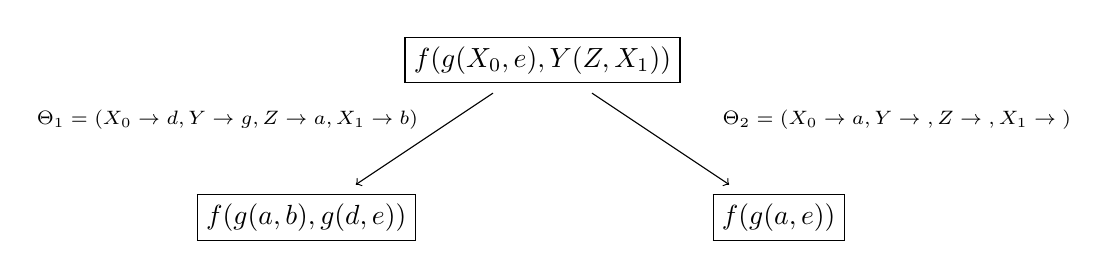
\begin{tikzpicture}
\node(au) at (5,2) {\fbox{\mbox{$f(g(X_0,e),Y(Z,X_1))$}}};
\node(left) at (2,0) {\fbox{\mbox{$f(g(a,b), g(d,e))$}}};
\node(right) at (8,0) {\fbox{\mbox{$f(g(a,e))$}}};
%
\draw[->](au) -- (left) node[pos=0.5, above]{\mbox{\scriptsize $\Theta_1 = ( X_0 \rightarrow d, Y \rightarrow g, Z \rightarrow a, X_1 \rightarrow b)$\hspace*{5cm}}};
\draw[->](au) -- (right) node[pos=0.5, above]{\mbox{\hspace*{6cm}\scriptsize $\Theta_2 = ( X_0 \rightarrow a, Y \rightarrow \NIL{}, Z \rightarrow \NIL{}, X_1 \rightarrow \NIL{})$}};
\end{tikzpicture}
\vspace*{1em}

\centering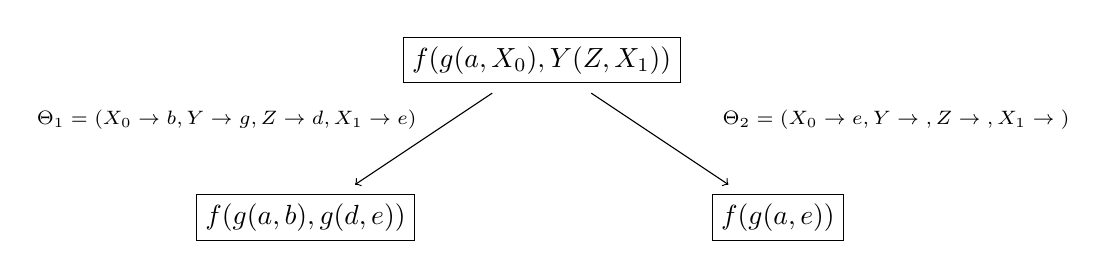
\begin{tikzpicture}
\node(au) at (5,2) {\fbox{\mbox{$f(g(a,X_0),Y(Z,X_1))$}}};
\node(left) at (2,0) {\fbox{\mbox{$f(g(a,b), g(d,e))$}}};
\node(right) at (8,0) {\fbox{\mbox{$f(g(a,e))$}}};
%
\draw[->](au) -- (left) node[pos=0.5, above]{\mbox{\scriptsize $\Theta_1 = ( X_0 \rightarrow b, Y \rightarrow g, Z \rightarrow d, X_1 \rightarrow e)$\hspace*{5cm}}};
\draw[->](au) -- (right) node[pos=0.5, above]{\mbox{\hspace*{6cm}\scriptsize $\Theta_2 = ( X_0 \rightarrow e, Y \rightarrow \NIL{}, Z \rightarrow \NIL{}, X_1 \rightarrow \NIL{})$}};
\end{tikzpicture}
\caption{Higher-order anti-unification modulo theories of the terms $f(g(a,b), g(d,e))$
and $f(g(a,e))$, creating multiple MSAs.}
  \label{fig:multipleMSA}
\end{figure}


Despite having multiple potential MSAs, we need to determine one single MSA that is the most appropriate in our context. However, the complexity of finding an optimal MSA is undecidable in general \cite{2008:fse:cottrell} since an infinite number of possible substitutions can be applied to every variable. Therefore, we need to use an approximation technique to construct one of the best MSAs that can sufficiently solve our problem.
% reason since?
%Our goal is to find an MSA that is an approximation of the best fit to our application

\section{Summary}  \label{summary}
We described abstract syntax trees (ASTs) as a standard syntactic representation of source code.  Every AST can also be represented in a function format (and vice versa) which constitute the standard theoretical concept of terms.  We demonstrated how the theoretical framework of anti-unification as a technique to construct a common generalization of two given terms, and hence of two ASTs.  First-order anti-unification permits terms to be replaced with variables and vice versa, but it is limited in that low-level commonality can be discarded due to high-level differences.  Higher-order anti-unification overcomes this by permit substitution relative to function symbols as well as terms.  A further extension allows for insertion and deletion by declaring equivalence with the \NIL{} structure, as well as other arbitrary equational theories to embed knowledge of semantic equivalence.  Unfortunately, this higher-order anti-unification modulo theories approach leads to ambiguity and the potential for an infinite number of possible substitutions for every structural variable.  To make use of that technique despite its weakness, we must apply an approximation technique to select amongst the best MSAs in order to reach a solution that is reasonable in practice.
